\documentclass{article}
\usepackage{amsmath}
\usepackage{amsfonts}
\usepackage{amssymb}
\usepackage{courier}
\usepackage{graphicx}
\usepackage{subfig}
\usepackage{listings}
\usepackage[margin=1in]{geometry}

\title{Visualization of Open Source Projects}
\begin{document}


\begin{titlepage}
    \begin{center}
        \vspace*{2.5cm}
        {\bf Visualization of Open Source Projects}
        
        \vspace{0.5cm}
        
        Analyzing trends in Github Organizations

        
        \vspace{4.0cm}        
        
        \textbf{David Leonard}
        
        \vspace{0.5cm}
        DrkSephy1025@gmail.com
        
        \vspace{3.0cm}
        
        \textbf{Liron Shimrony}
        \vspace{0.5cm}
        
        lsxliron@gmail.com
        
	
	\vspace{2.5cm} 
	Date: May 1, 2016
        
        \vspace{1in}
        \vfill
        
    \end{center}
\end{titlepage}

\tableofcontents

\newpage

\section {Introduction}

One of the biggest and most interesting data sources online is \textbf{source code} stored in various version control platforms, such as \textbf{Github} and \textbf{Bitbucket}. These platforms contain various projects stored in \textbf{repositories}, which contain various metadata with which we can draw several conclusions from. This metadata consists of metrics such as:

\begin{itemize}
	\item \textbf{Commits}: Snapshots of the codebase at a given point in time.
	\item \textbf{Issues}: Feature requests and bug reports for a given project.
	\item \textbf{Pull Requests}: Code patches submitted by various other contributors  around the world.
\end{itemize}

The challenge here is to discover various trends in the data with which may not be visible depending on the visualizations chosen to represent the data. However, it is infeasible to analyze every single repository across Github or Bitbucket for this project - as the number of repositories is in the millions. In order to draw meaningful conclusions from the data, we will be selectively analyzing open source projects on Github pertaining to the \textbf{Facebook} organization. The choice for this is arbitrary, but we chose Facebook because it is responsible for open sourcing various projects in the last few years which have heavily influenced the open source community. From this data, we expect to draw various conclusions regarding the lifespan of their open source projects and how they progress over time.

\section {Why?}

Given the general form of the data, the big challenge is to come up with a meaningful visualization which allows us to derive some conclusions.  There have been several projects which strictly visualize \textbf{commits} in a given repository, which typically generate a tree-like structure (or a structure in general). These visualizations show how large a project gets over the course of time as the number of developers and commits increases. While the structures that are generated at the end of these visualizations are interesting to look at, it is difficult to draw any sort of meaningful conclusions. In the next few sections, we briefly show some popular works in this domain.

\subsection {Code Swarm}

Code Swarm [2] is a visualization of commits in a repository, which was also created by Michael Ogawa [1]. Code Swarm represents files as moving elements, where both files are mapped to the developer which created it. Moreover, these files are color coded based on whether or not they are source code or general documents. When developers drop off in their contributions, they fade over time from the underlying histogram at the bottom which allows us to keep track of what events have occurred before in the timeline. Code Swarm is able to visualize a wide spectrum of repository types: 

\begin {itemize}
	\item {Subversion}
	\item {CVS}
	\item {Git}
	\item {Mercurial}
	\item {Perforce}
	\item {VSS}
	\item {Starteam}
	\item {Wikiswarm}
	\item {Darcs}
\end {itemize}

\begin{figure}[h!]
\centering
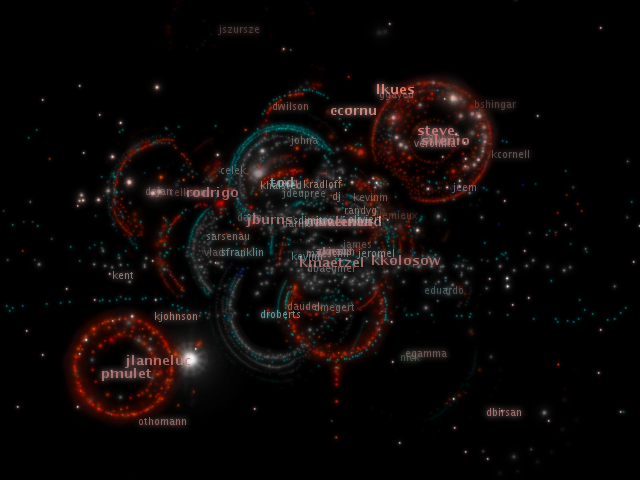
\includegraphics[height=8cm, width=12cm]{swarm}
\caption{Code Swarm}
\end{figure}

\subsection {Gource}

Another popular source code visualization tool is \textbf{Gource}, which also generates a tree-like structure of the repository similar to Code Swarm. Gource is able to visualize \textbf{git}, \textbf{subversion}, \textbf{mercurial} and \textbf{bazaar} repositories. These visualizations consist of the root directory being mapped to the root of the tree, while directories will become branches and subsequent files become leaf nodes as time elapses from the conception of the repository to the last commit. 

\begin{figure}[h!]
\centering
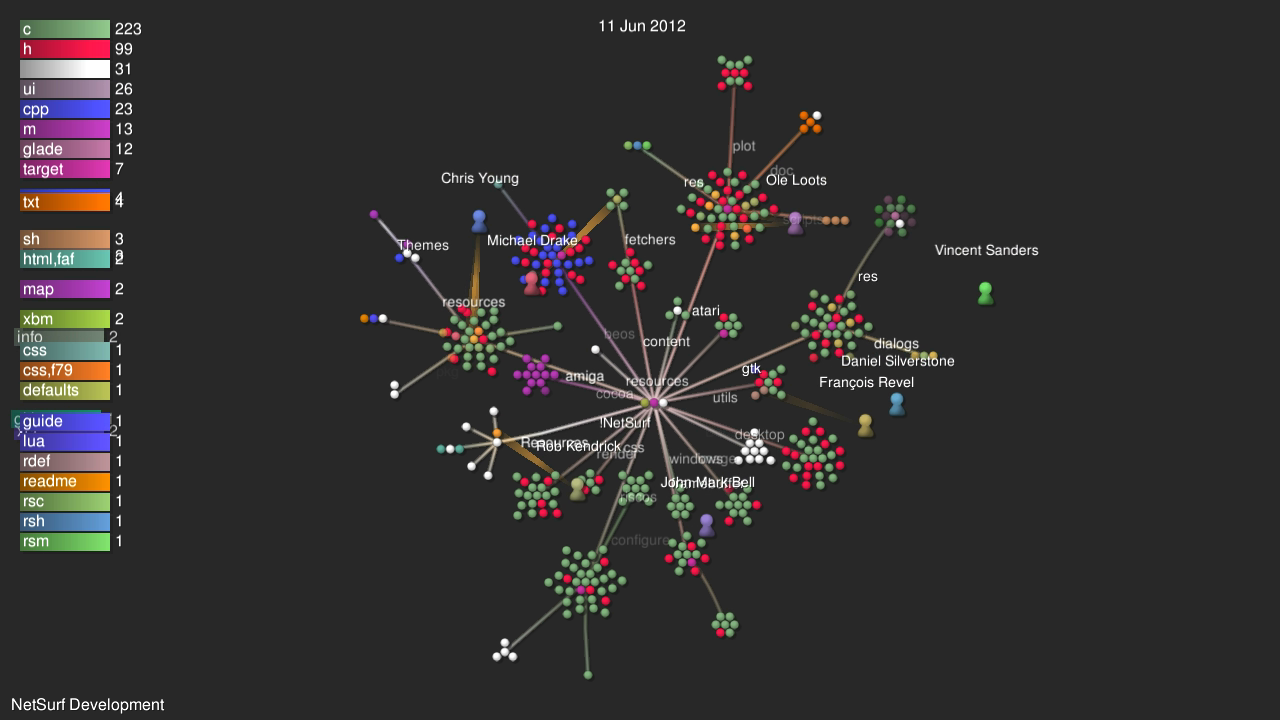
\includegraphics[height=8cm, width=12cm]{gource}
\caption{Gource Visualization}
\end{figure}

\subsection {Github Visualizer}

One of the most comprehensive open source visualization tools is \textbf{Github Visualizer}[4], which was built using d3\footnote{d3: https://d3js.org/} and the Github API\footnote{Github API: https://developer.github.com/v3/}. Using this tool, one may visualize events in a Github repository ranging from commits to lines of code over time. During the runtime of the visualization, a histogram is built along the time-axis showing the density of events for the current time frame. Moreover, a user may choose to visualize an individual repository belonging to a user, or they may visualize all repositories which belong to a given user. By hovering over various elements in the visualization, we can drill down deeper and analyze the lines of code that are added over time per time series event. For reference, we have included a visualization of Facebook repositories generated by this tool in Figure 3.

\begin{figure}[h!]
\centering
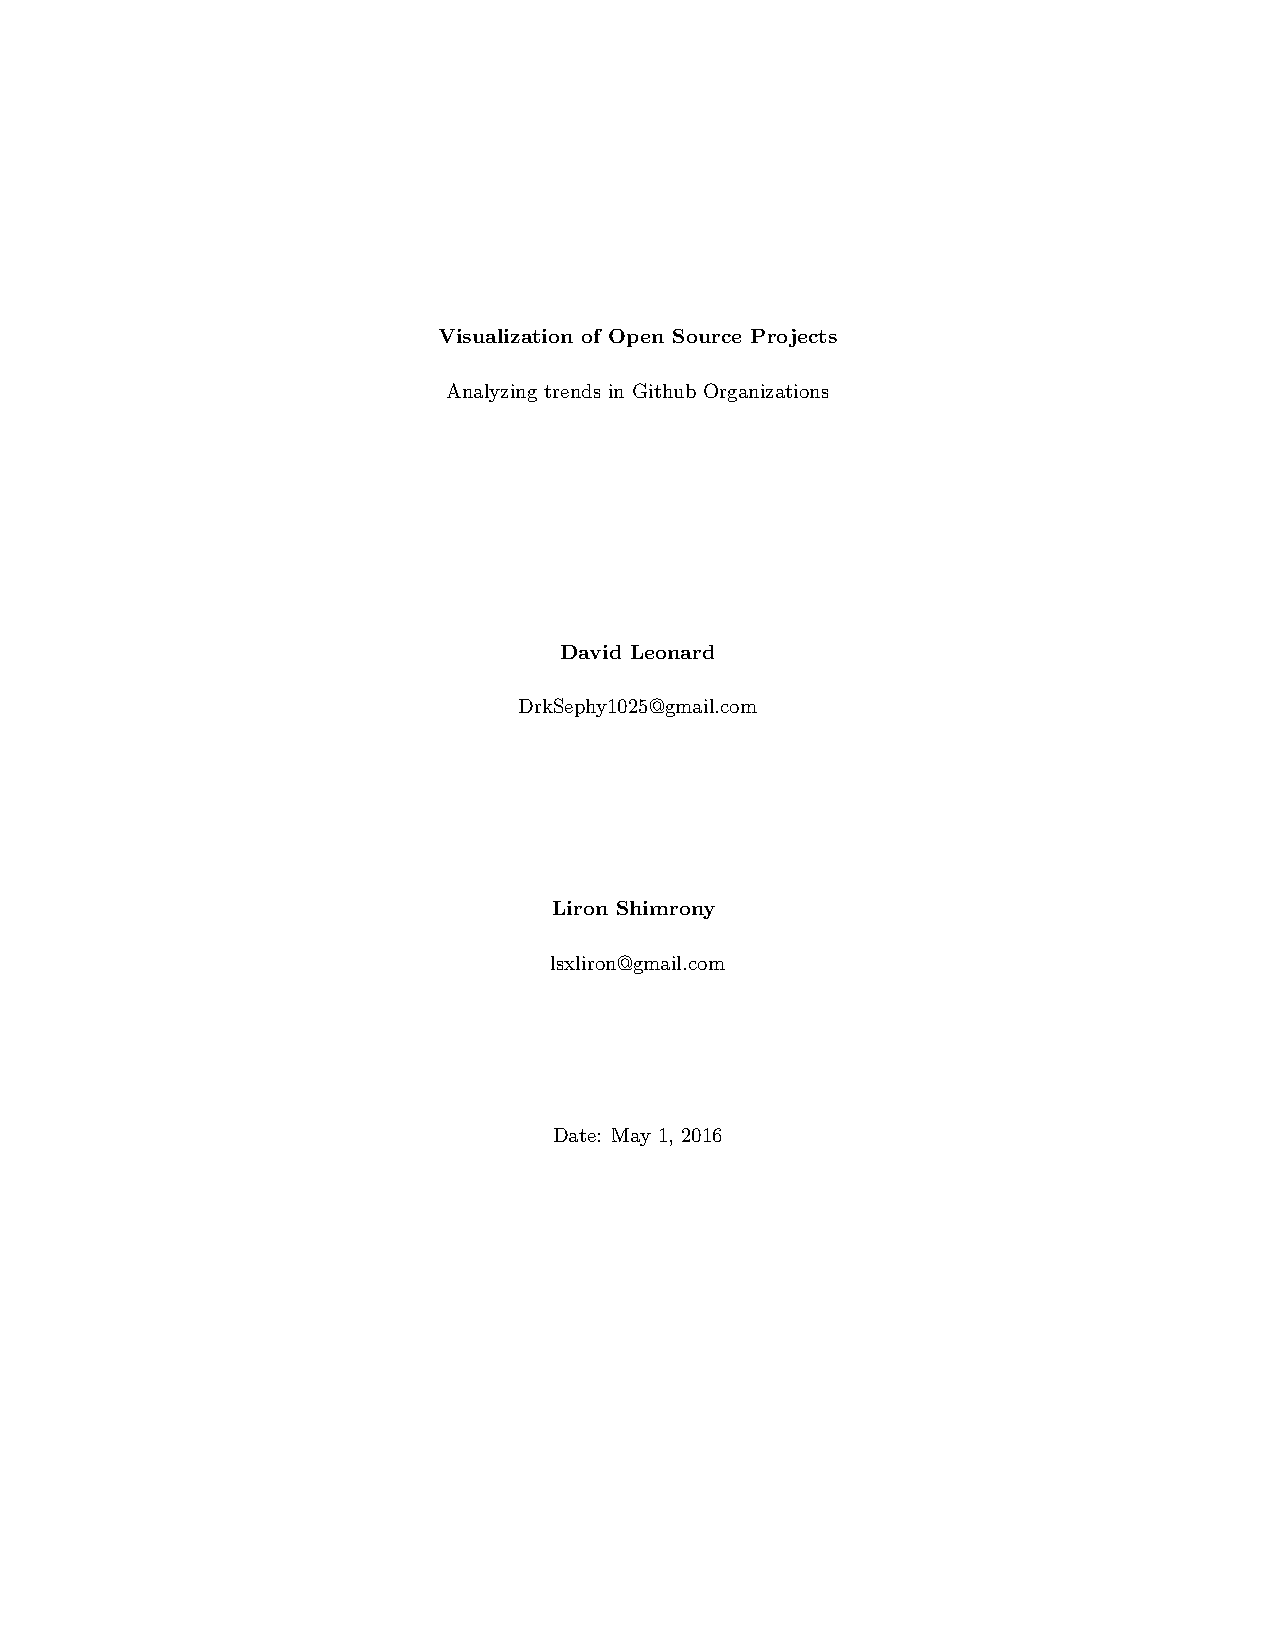
\includegraphics[height=10cm, width=16cm]{viz}
\caption{Github Visualizer: Facebook Repositories}
\end{figure}

While this visualization is very interesting to look at, we fell that it is too dense and it becomes a challenge to narrow down on a particular aspect of the visualization. It is hard to draw any solid conclusions from what is presented, and trends are hard to discover apart from the event density histogram. In our own project, we aim to build a series of visualizations which are simple yet powerful with respect to the trends that can be discovered.

\section {What?}

In this section we discuss the visualizations which we have created over the span of this project. As mentioned earlier, this project was created without knowing the questions we want to answer, but we expect several noticeable trends to crop up throughout the lifespan of these open source projects. We begin by discussing our first visualization: the \textbf{event bar chart}.

\subsection {Event Bar Chart}

Our first goal was to show the sum totals of various events 

\subsection {Event Time Series}

\subsection {Repository Treemap}

\subsection {Interactivity}

\section {How?}

\section {So What?}

\section {Conclusion}

\newpage

\begin{thebibliography}{9}
 
\bibitem{einstein} 
Michael Ogawa, and Kwan-Liu Ma
\textit{Software evolution storylines}.
Proceedings of the 5th international symposium on Software visualization. ACM, 2010.

\bibitem{einstein} 
Michael Ogawa.
\textit{Code Swarm}.
http://vis.cs.ucdavis.edu/~ogawa/codeswarm/

\bibitem{einstein} 
Andrew Caudwell.
\textit{Gource}.
https://github.com/acaudwell/Gource

\bibitem{einstein} 
Artem  Zubkov.
\textit{Github Visualizer}.
http://ghv.artzub.com/

\end{thebibliography}

\end{document}
